%\documentclass[handout]{beamer}
\documentclass{beamer}
\usepackage[utf8]{inputenc}
\usepackage[francais]{babel}
\usepackage[T1]{fontenc}
%\usepackage{multimedia}
\usepackage{graphicx}
\usepackage{hyperref}
\usepackage{algorithm}
\usepackage{algpseudocode}
\floatname{algorithm}{Algorithme} 
\usepackage{listings}

%\usetheme[width=100pt]{PaloAlto}
\usetheme[compress]{Ilmenau}
%\usecolortheme{fly}
\setbeamertemplate{frametitle}[default][center]

%\setbeamercovered{transparent}

\title{Proactive : Un middleware open source pour le calcul parallèle}

\author{Veyssier Julien}
\institute{CBGP - INRA}
\date{25 Octobre 2011}
\setbeamertemplate{navigation symbols}{}
%\logo{}
\begin{document}

\begin{frame}
\titlepage
\end{frame}

\begin{frame}
\tableofcontents
\end{frame}

\section[Introduction]{Introduction}
\begin{frame}
	\tableofcontents[currentsection]
\end{frame}

\begin{frame}{Contexte}
	\begin{columns}
	\begin{column}[l]{0.5\linewidth}
        \begin{columns}
        \begin{column}[l]{0.5\linewidth}
        \begin{figure}
            %[!bh]
            \centering
            
\includegraphics[scale=0.32]{cbgp.png}
            %\caption{Architecture autour d'un CDN}
        \end{figure}
        \end{column}
        \begin{column}[r]{0.5\linewidth}
        \begin{figure}
            %[!bh]
            \centering
            
\includegraphics[scale=0.32]{cocci.png}
            %\caption{Architecture autour d'un CDN}
        \end{figure}
        \end{column}
        \end{columns}
        \vspace{1cm}
	\begin{block}{Objectifs}<2->
			\begin{itemize}
                    %decouplage .. .
                \item Refonte de DIYABC
				\item Implémentation de l'interface graphique
                \item Interfaçage avec des outils de calcul parallèle
			\end{itemize}
					
		\end{block}

	\end{column}
	\begin{column}[r]{0.5\linewidth}
	\begin{exampleblock}{Activités du laboratoire}<1->
			\begin{itemize}
				\item Génétique des population
                \item Systématique
                \item Écologie
			\end{itemize}
					
		\end{exampleblock}
	\begin{block}{Moyens matériels}<3->
			\begin{itemize}
                \item Cluster local (SGE)
				\item Machines personnelles des chercheurs
                \item Postes de travail de l'administration
			\end{itemize}
					
		\end{block}
	\end{column}
	\end{columns}
\end{frame}

\begin{frame}{État de l'art}
    Constat : architectures trop rigides et fastidieuses à maintenir
	\begin{columns}
	\begin{column}[l]{0.3\linewidth}
    \begin{block}{Projets}
        \begin{itemize}
            \item<2-> Diane
            \item<3-> Ganga
            \item<4-> Wisdom
            \item<5-> OurGrid
            \item<6-> Proactive
        \end{itemize}
    \end{block}
	\end{column}
	\begin{column}[r]{0.6\linewidth}
    \begin{exampleblock}{Particularité}
        \begin{itemize}
            \item<2-> Peu d'outils annexe
            \item<3-> Sous-partie de DIANE
            \item<4-> Orienté vers les grilles de calcul
            \item<5-> Programmes non fournis
            \item<6-> Découplé et polyvalent
        \end{itemize}
    \end{exampleblock}
	\end{column}
	\end{columns}
\end{frame}

\begin{frame}{Proactive}
    Exploration des possibilités pour une éventuelle intégration au CBGP
\end{frame}

\section[Fonctionnement]{Fonctionnement de Proactive}
\begin{frame}{Caractéristiques}
    Langage de programmation $\Longrightarrow$ Java + Bash/Batch
    Portable
    Supporte un environnement hétérogène%on y reviendra plus tard

\end{frame}
\subsection{Architecture}
\begin{frame}{Architecture}
	\begin{columns}
	\begin{column}[l]{0.5\linewidth}
        \begin{figure}
            %[!bh]
            \centering
            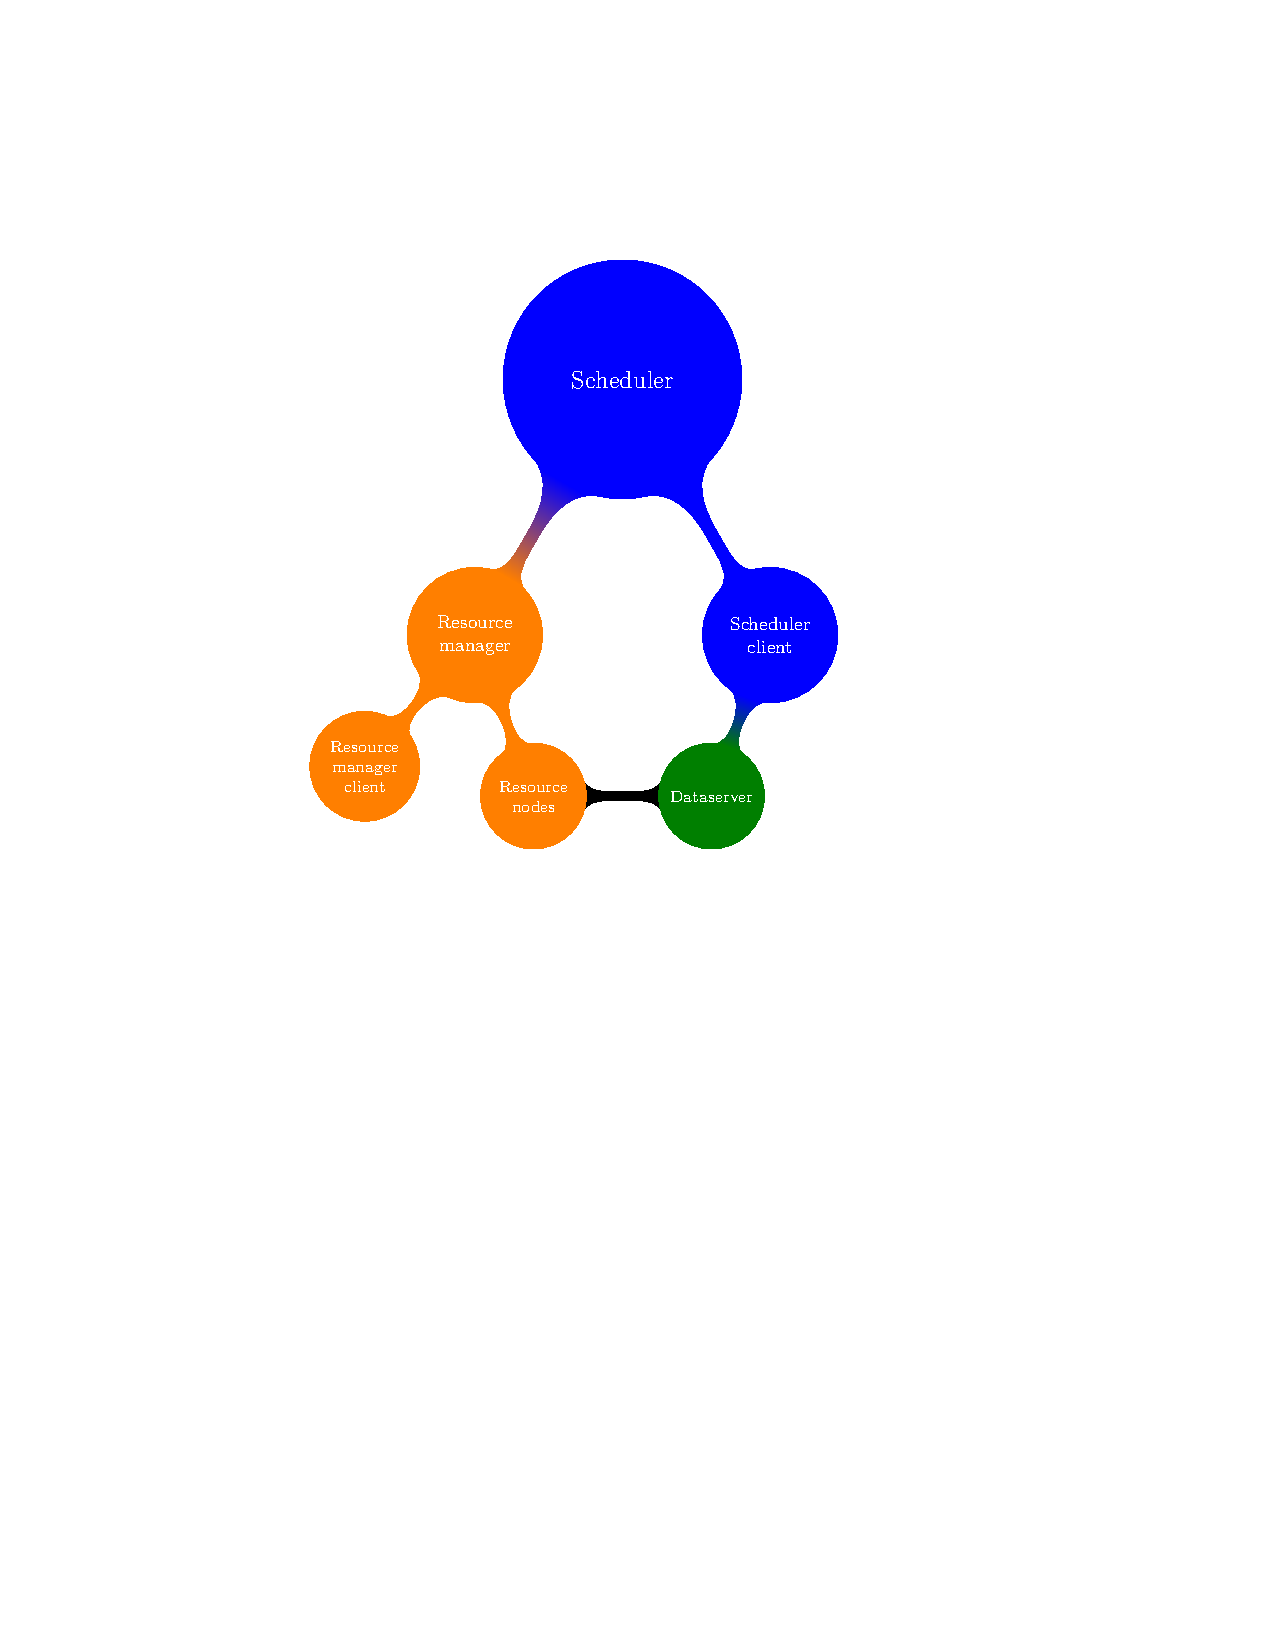
\includegraphics[trim=4cm 13cm 2cm 5cm,scale=0.48]{netmap_abs.pdf}
            \caption{Communication dans Proactive}
        \end{figure}
	\end{column}
    \setbeamercolor{block title}{fg=black,bg=orange}   
    \setbeamercolor{block body}{fg=black,bg=orange!30}
    \setbeamercolor{block title alerted}{fg=black,bg=blue}   
    \setbeamercolor{block body alerted}{fg=black,bg=blue!30}
    \setbeamercolor{block title example}{fg=black,bg=green!50!black}   
    \setbeamercolor{block body example}{fg=black,bg=green!20}
	\begin{column}[r]{0.5\linewidth}
        \begin{block}{Resource management}
            Gestion des noeuds de calcul
        \end{block}
        \begin{alertblock}{Scheduler}
             Gestion de la politique d'ordonnancement et de la soumission des t\^aches
        \end{alertblock}
        \begin{exampleblock}{Data management}
            Transmission des données
        \end{exampleblock}
        
	\end{column}
	\end{columns}
\end{frame}

\subsection{Composants}
\begin{frame}{Programmes}
	\begin{columns}
	\begin{column}[l]{0.5\linewidth}
        \begin{figure}
            %[!bh]
            \centering
            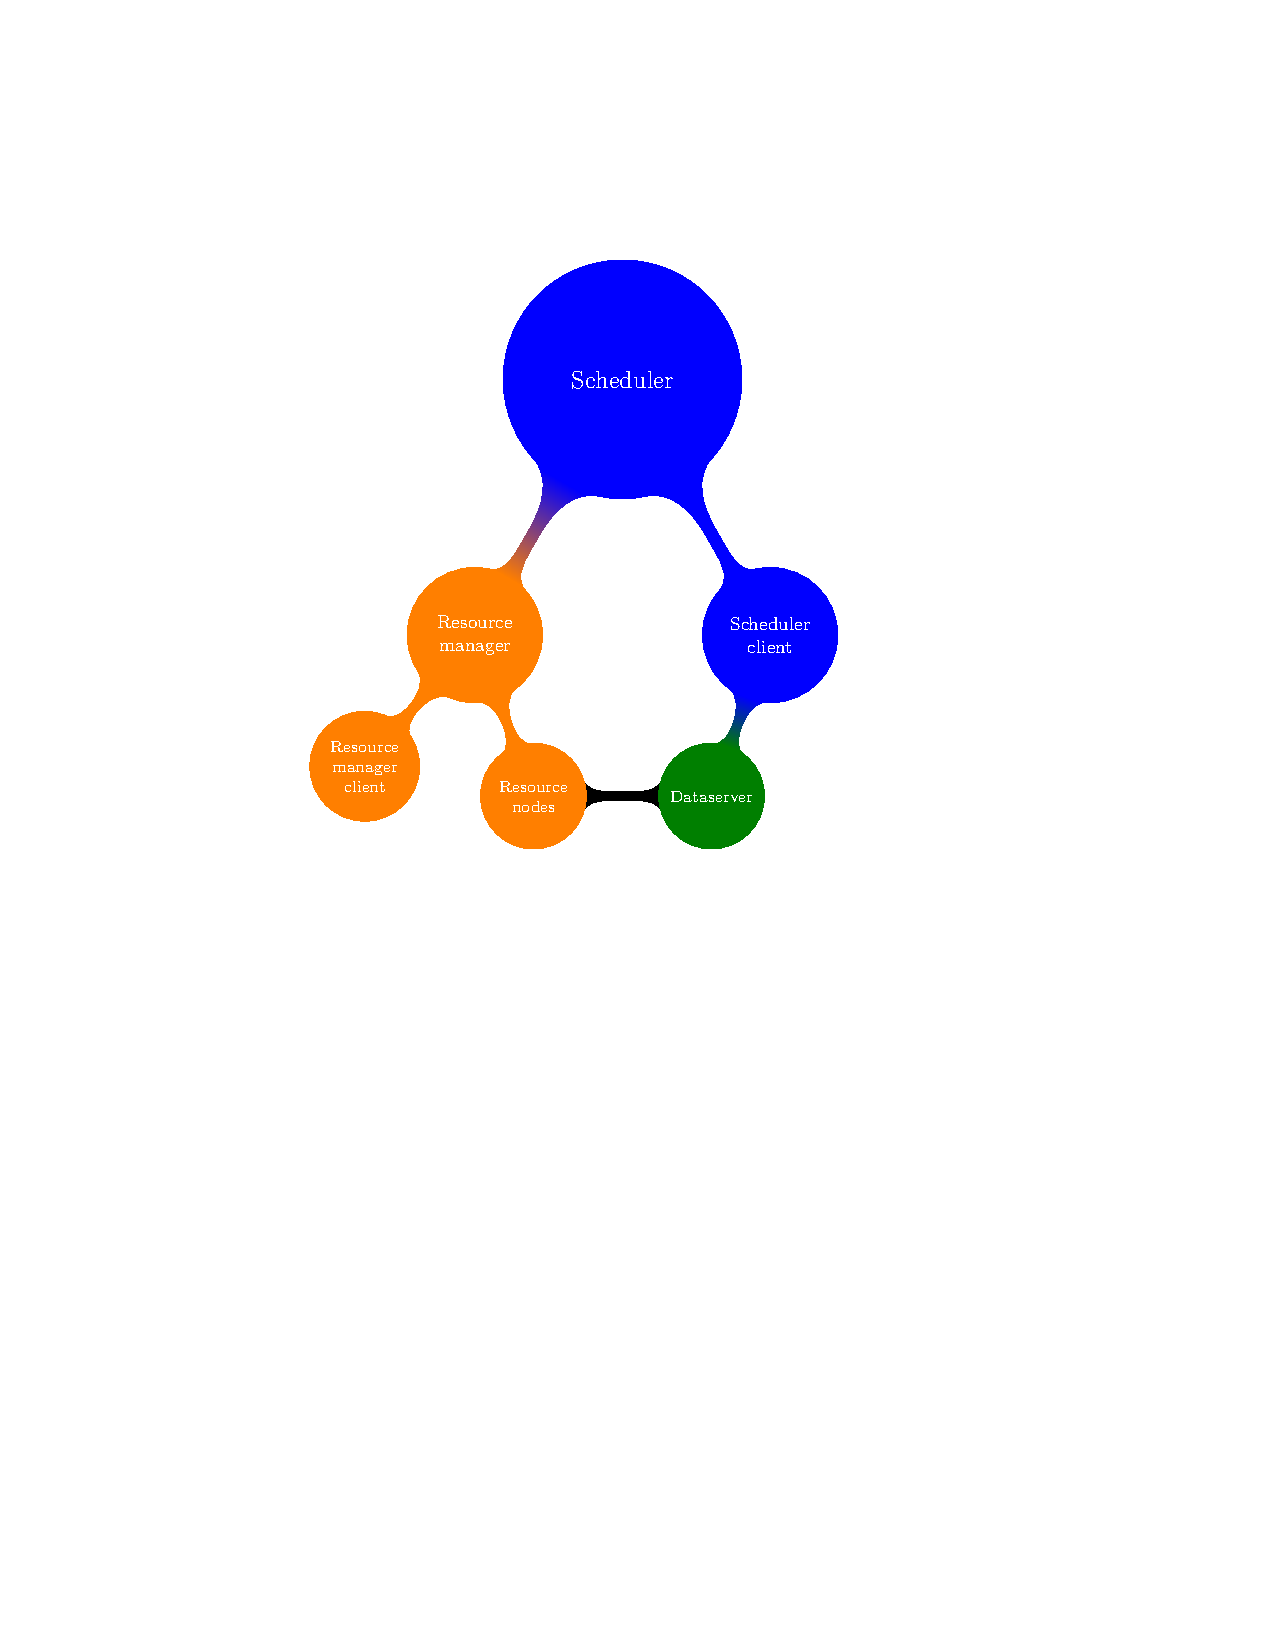
\includegraphics[trim=4cm 13cm 2cm 5cm,scale=0.48]{netmap_abs.pdf}
            \caption{Communication dans Proactive}
        \end{figure}
	\end{column}
    \setbeamercolor{block title}{fg=black,bg=orange}   
    \setbeamercolor{block body}{fg=black,bg=orange!30}
    \setbeamercolor{block title alerted}{fg=black,bg=blue}   
    \setbeamercolor{block body alerted}{fg=black,bg=blue!30}
    \setbeamercolor{block title example}{fg=black,bg=green!50!black}   
    \setbeamercolor{block body example}{fg=black,bg=green!20}
	\begin{column}[r]{0.5\linewidth}
        
        \begin{block}{Resource node}
            Accepte et traite des t\^aches
        \end{block}
        \begin{block}{Resource manager}
            Contrôle les noeuds de calcul
        \end{block}
        \begin{alertblock}{Scheduler}
            Attend des t\^aches et les affecte à des noeuds de calcul
        \end{alertblock}
        \begin{exampleblock}{Dataserver}
            Transmet les données liées aux calculs
        \end{exampleblock}
        
	\end{column}
	\end{columns}
\end{frame}

\begin{frame}{Resource node et Resource manager}
	\begin{columns}
	\begin{column}[l]{0.5\linewidth}
        \begin{figure}
            %[!bh]
            \centering
            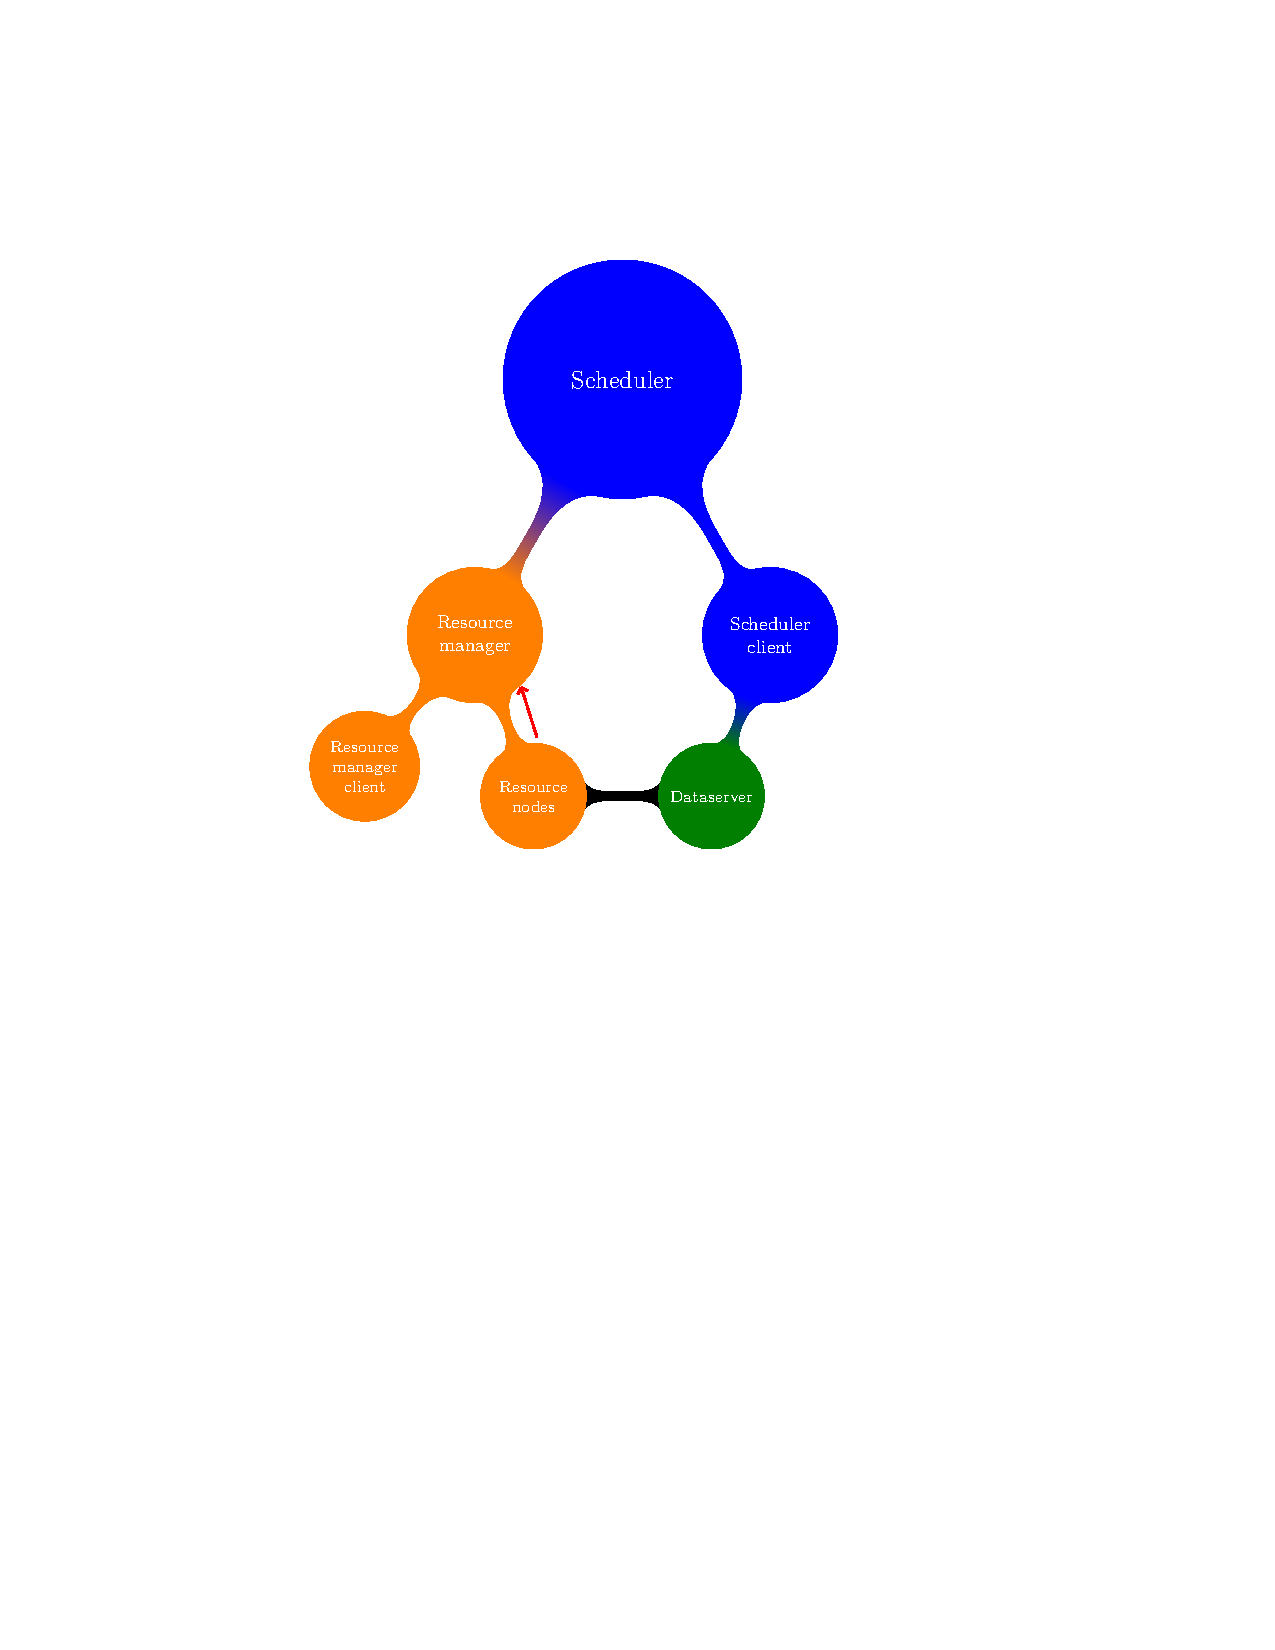
\includegraphics[trim=4cm 13cm 2cm 5cm,scale=0.48]{node_declaration.pdf}
            \caption{Communication dans Proactive}
        \end{figure}
	\end{column}
    \setbeamercolor{block title}{fg=black,bg=orange}   
    \setbeamercolor{block body}{fg=black,bg=orange!30}
    \setbeamercolor{block title alerted}{fg=black,bg=blue}   
    \setbeamercolor{block body alerted}{fg=black,bg=blue!30}
	\begin{column}[r]{0.5\linewidth}
        
        \begin{block}{Resource node}<1->
             a lancer sur chaque machine ressource
             reçoit les taches, les execute dans un env temporaire qui sera nettoyé
        \end{block}
        \begin{block}{Resource manager}<2->
             attend la connexion des noeuds de calcul et les requêtes de l'ordonnanceur
        \end{block}
	\end{column}
	\end{columns}
\end{frame}

\begin{frame}{Dataserver}
	\begin{columns}
	\begin{column}[l]{0.5\linewidth}
        \begin{figure}
            %[!bh]
            \centering
            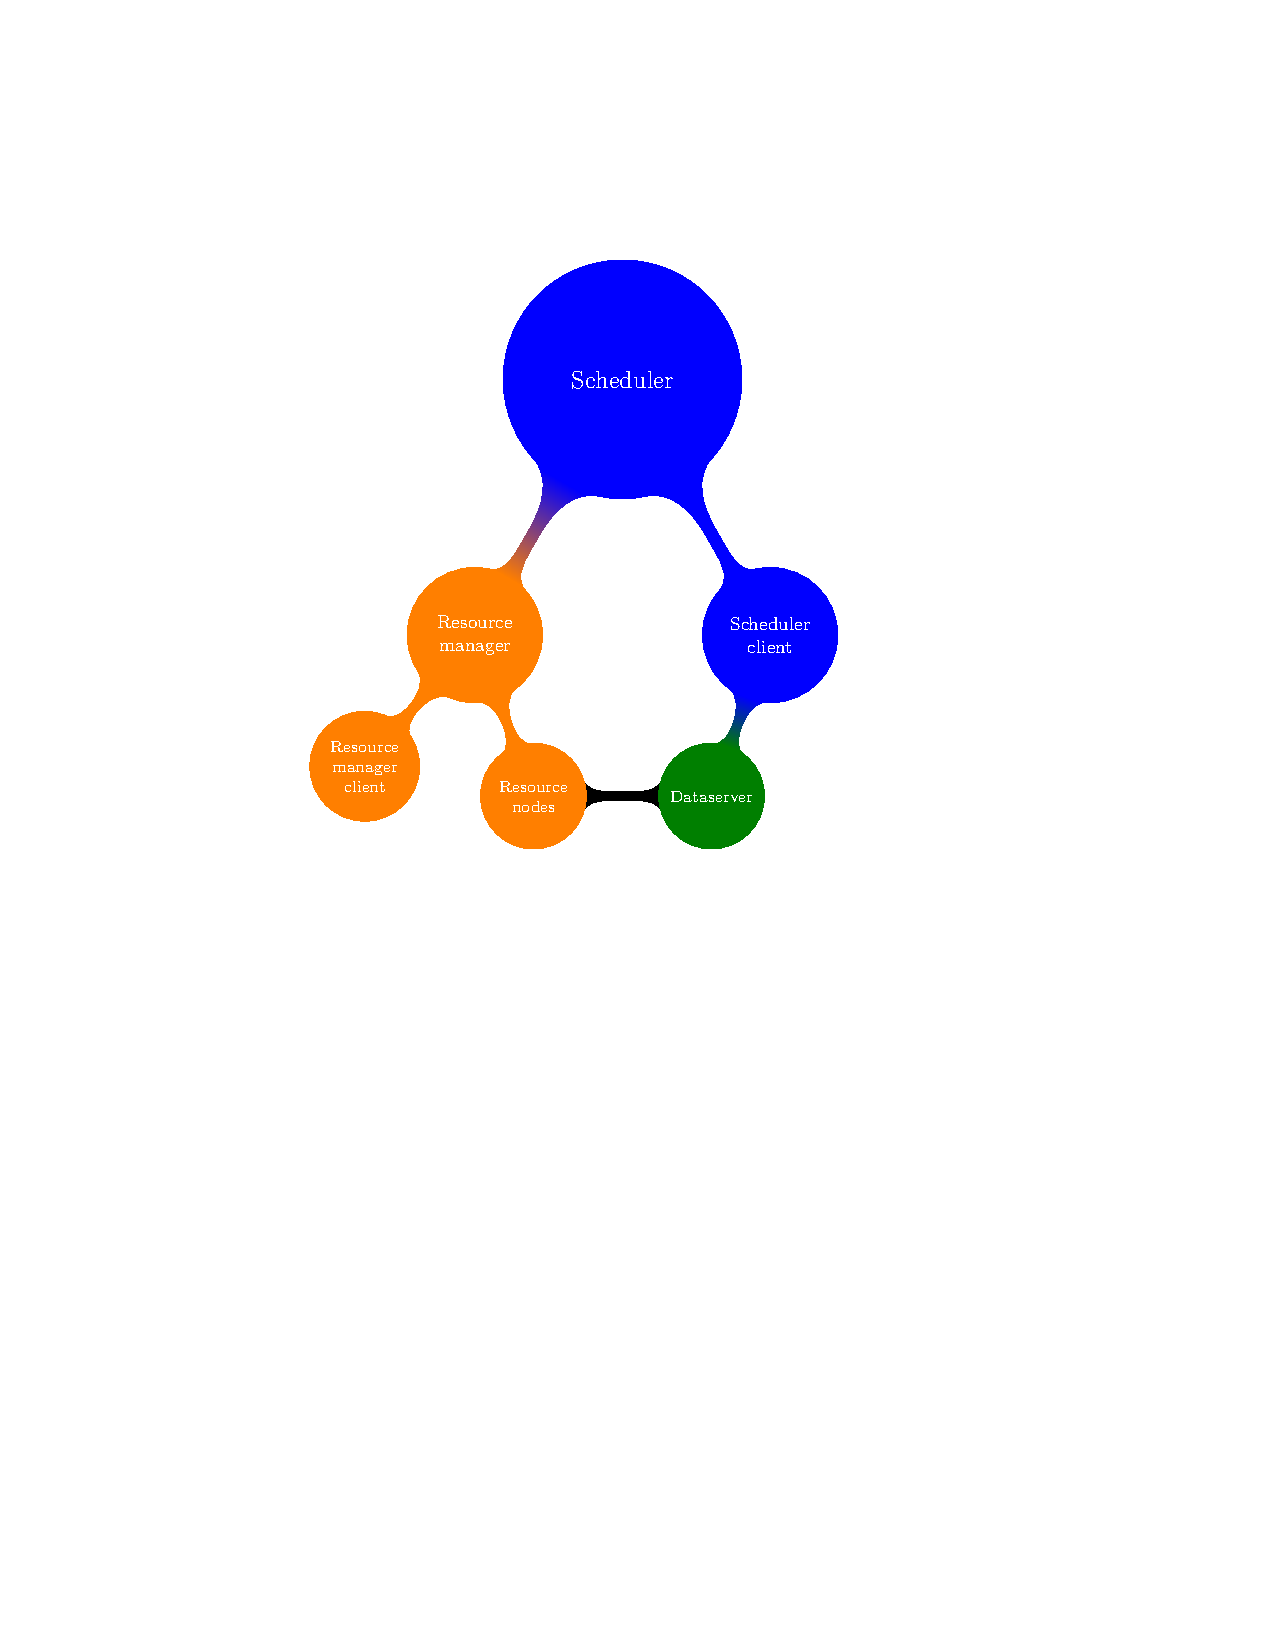
\includegraphics[trim=4cm 13cm 2cm 5cm,scale=0.48]{netmap_abs.pdf}
            \caption{Communication dans Proactive}
        \end{figure}
	\end{column}
    \setbeamercolor{block title example}{fg=black,bg=green!50!black}   
    \setbeamercolor{block body example}{fg=black,bg=green!20}
	\begin{column}[r]{0.5\linewidth}
        \begin{exampleblock}{Dataserver}
             Crée un espace accessible en lecture et en écriture

             Peut être lancé par un administrateur pour fournir un espace permanent commun à tous les utilisateurs (faisable au CBGP, petite taille)
             peut être lancé par chaque client pour créer l'espace sur sa propre machine
             Plusieurs client peuvent avoir accès au même espace
            
        \end{exampleblock}
        
	\end{column}
	\end{columns}
    
\end{frame}

\begin{frame}{Ordonnanceur (Scheduler)}
	\begin{columns}
	\begin{column}[l]{0.5\linewidth}
        \begin{figure}
            %[!bh]
            \centering
            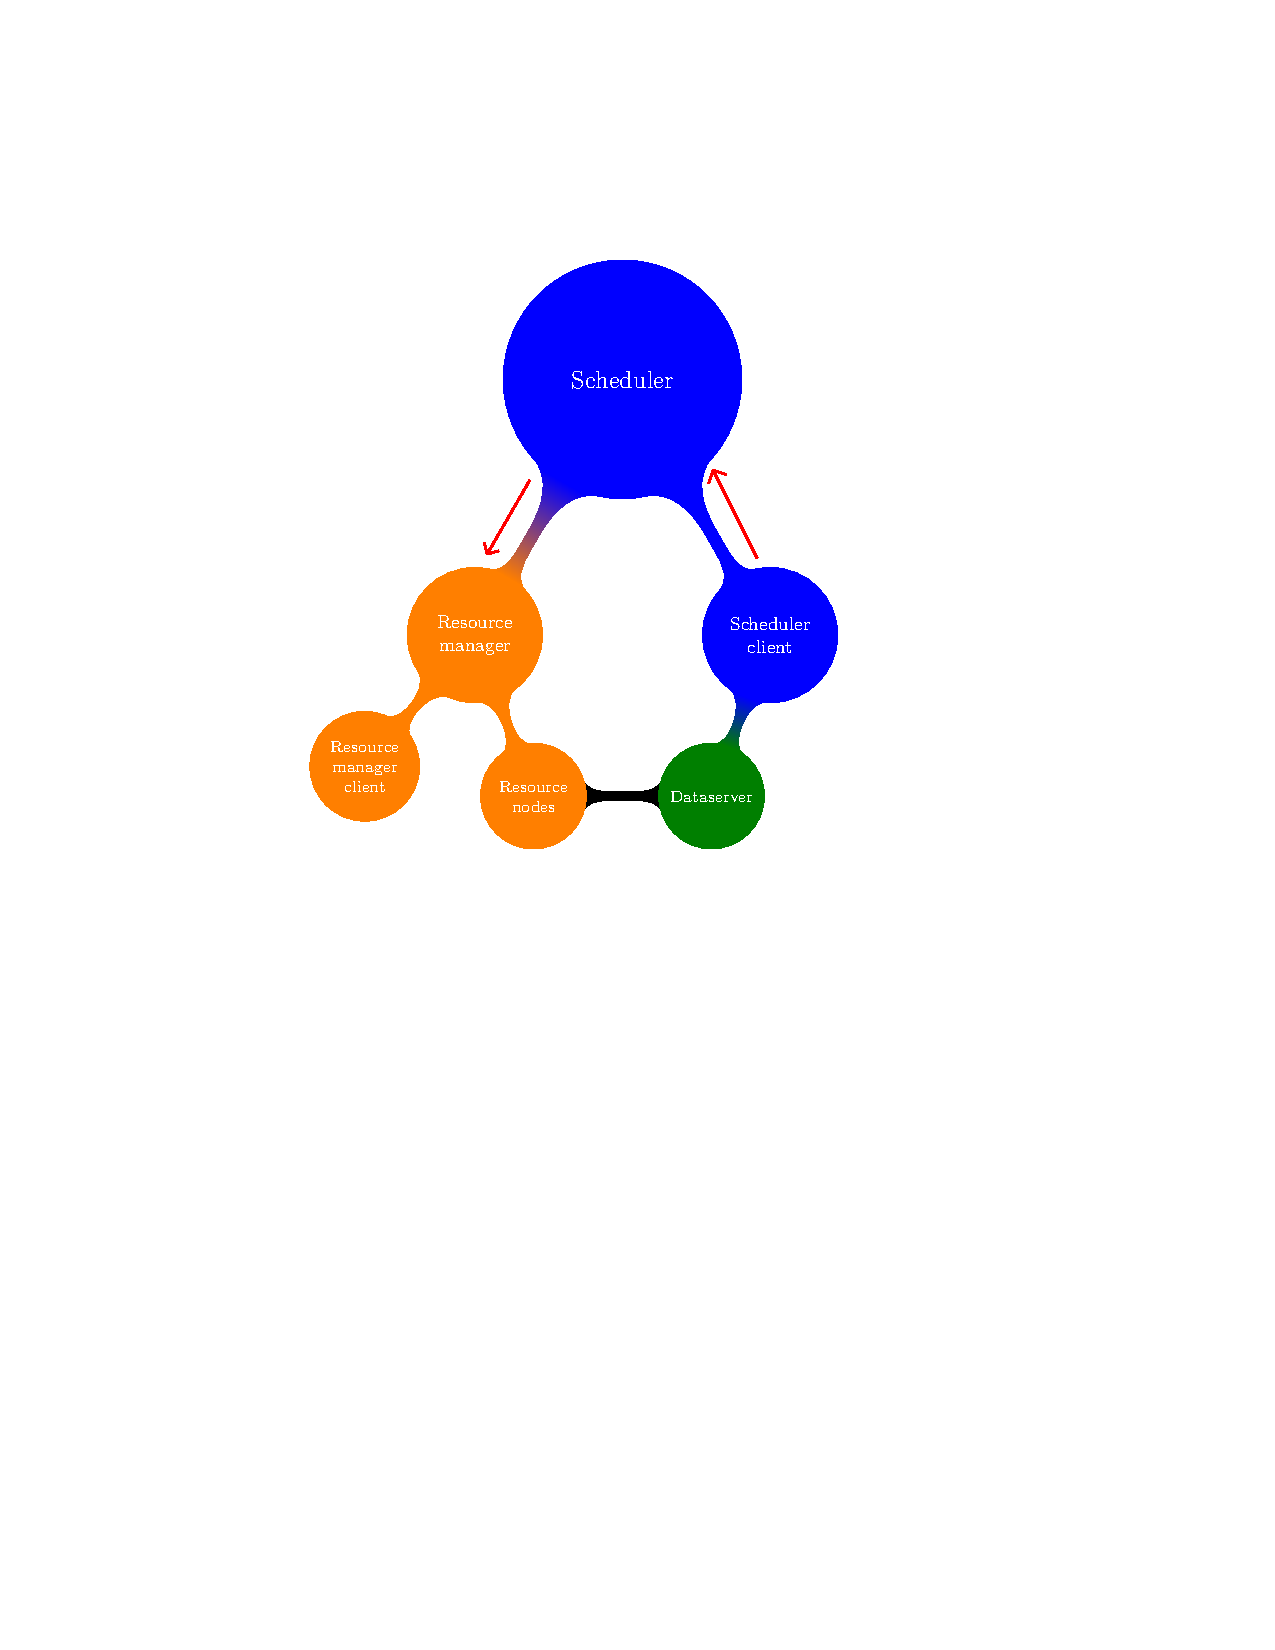
\includegraphics[trim=4cm 13cm 2cm 5cm,scale=0.48]{submit.pdf}
            \caption{Communication dans Proactive}
        \end{figure}
	\end{column}
    \setbeamercolor{block title}{fg=black,bg=orange}   
    \setbeamercolor{block body}{fg=black,bg=orange!30}
    \setbeamercolor{block title alerted}{fg=black,bg=blue}   
    \setbeamercolor{block body alerted}{fg=black,bg=blue!30}
	\begin{column}[r]{0.5\linewidth}
        \begin{block}{Scheduler}
             est l'intermédiaire entre le client et le gestionnaire de ressources
             Il gère l'authentification des clients et leurs droits d'accès aux ressources 
             et sait communiquer avec le rm pour affecter les taches aux noeuds de calcul
        \end{block}
        
	\end{column}
	\end{columns}
    
\end{frame}

\subsection{Architecture}

\begin{frame}{Communication dans Proactive}
    \begin{figure}
        %[!bh]
        \centering
        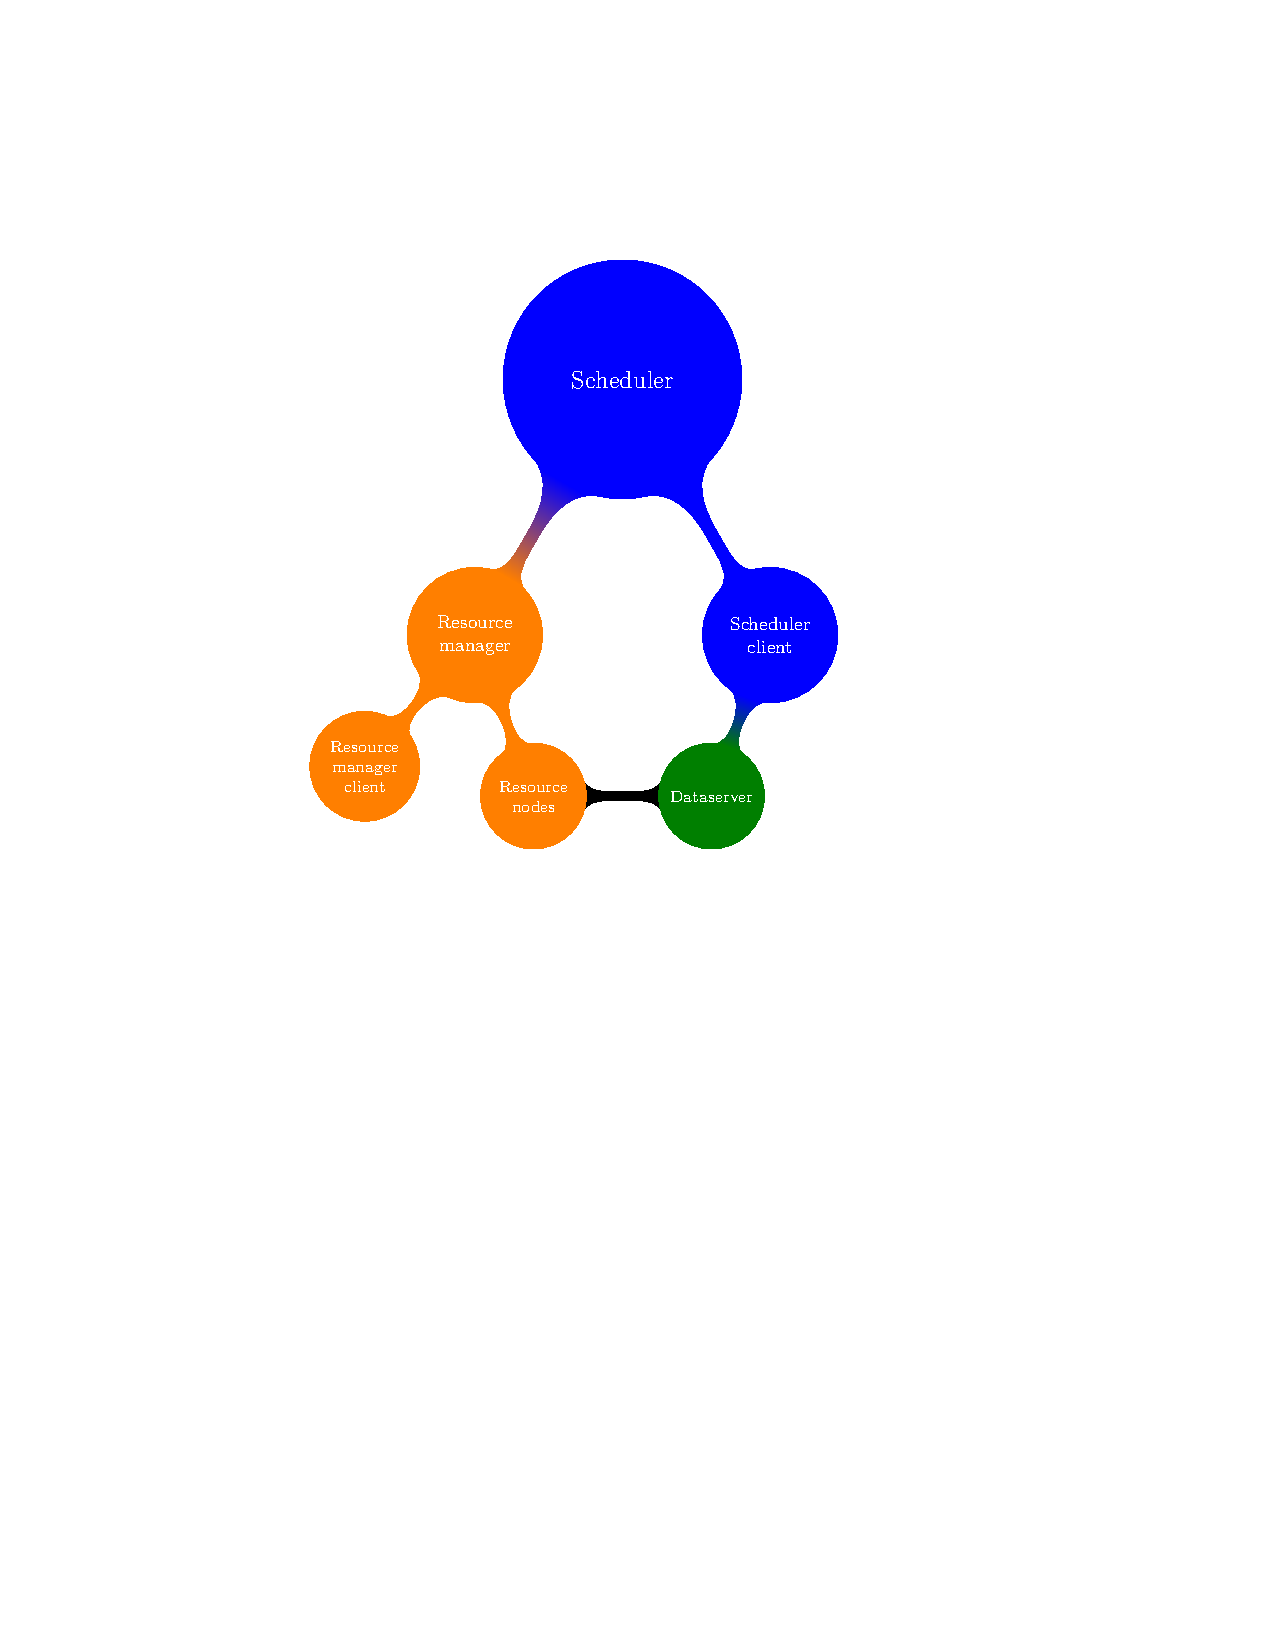
\includegraphics[trim=4cm 13cm 4cm 4cm,scale=0.62]{netmap_abs.pdf}
        %\caption{Principe de communication dans le réseau Proactive}
    \end{figure}
    
\end{frame}

\subsection{Définition d'une tache}
\begin{frame}
        \begin{block}{Qu'est-ce qu'une t\^ache ?}
        % en java, par xml, ou par liste de commandes
            \begin{itemize}
                \item Un identifiant
                \item Un serveur de données
                \item Une liste d'opération à effectuer %option dependances, retry..
            \end{itemize}
        \end{block}
\end{frame}

\begin{frame}{Avec une liste de commandes natives}
	\begin{columns}
	\begin{column}[l]{0.4\linewidth}
        \begin{exampleblock}{liste}
            \begin{itemize}
                \item Liste de commandes qui seront exécutées directement sur un noeud de calcul
                \item Gestion basique
            \end{itemize}
        \end{exampleblock}
	\end{column}
	\begin{column}[r]{0.6\linewidth}
        /path/to/script\_1.sh arg1 arg2\newline
        /path/to/script\_2.sh arg3 arg4\newline
        /path/to/script\_3.sh arg5 arg6\newline
	\end{column}
	\end{columns}
    
\end{frame}
\begin{frame}{En XML}
	\begin{columns}
	\begin{column}[l]{0.4\linewidth}
        \begin{exampleblock}{Définition par XML}
            \begin{itemize}
                \item Fichier XML qui spécifie chaque paramètre
                \item Plus simple mais moins complète que Java
            \end{itemize}
        \end{exampleblock}
	\end{column}
	\begin{column}[r]{0.6\linewidth}
        \vspace{-1cm}
        \begin{figure}
            %[!bh]
            \centering
            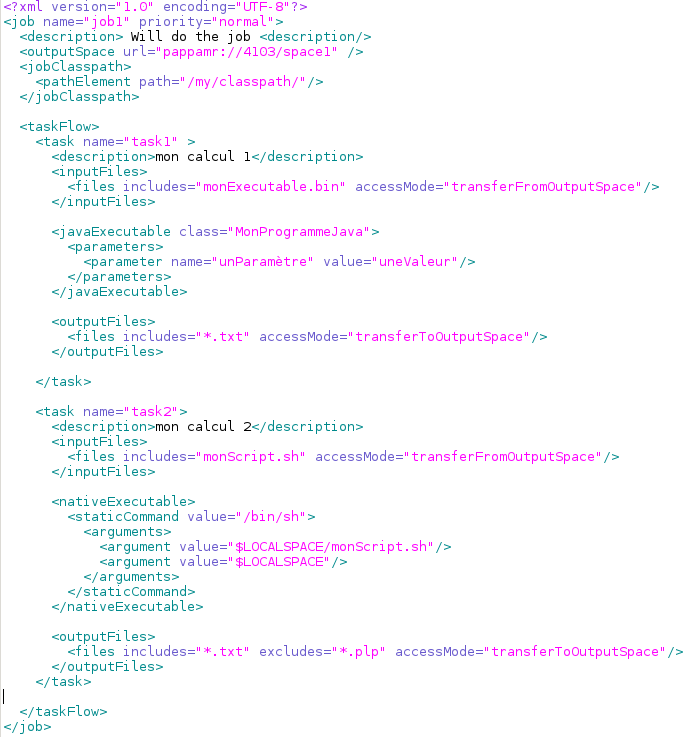
\includegraphics[scale=0.27]{jobxml.png}
            %\caption{Communication dans Proactive}
        \end{figure}
	\end{column}
	\end{columns}
    
\end{frame}
\begin{frame}{En Java}
	\begin{columns}
	\begin{column}[l]{0.4\linewidth}
        \begin{exampleblock}{Définition dans un programme en Java}
            \begin{itemize}
                \item Directement dans un programme en Java qui se connecte au scheduler
                \item Gestion fine
            \end{itemize}
        \end{exampleblock}
	\end{column}
	\begin{column}[r]{0.6\linewidth}
        \vspace{-1cm}
        \begin{figure}
            %[!bh]
            \centering
            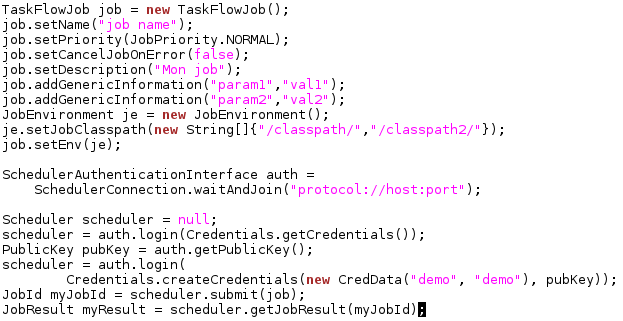
\includegraphics[scale=0.32]{jobjava.png}
            %\caption{Communication dans Proactive}
        \end{figure}
	\end{column}
	\end{columns}
    
\end{frame}

\subsection{Outils graphiques}
\begin{frame}{Scheduler client}
    % interessant pour la partie job submission et job results
    \begin{figure}
        %[!bh]
        \centering
        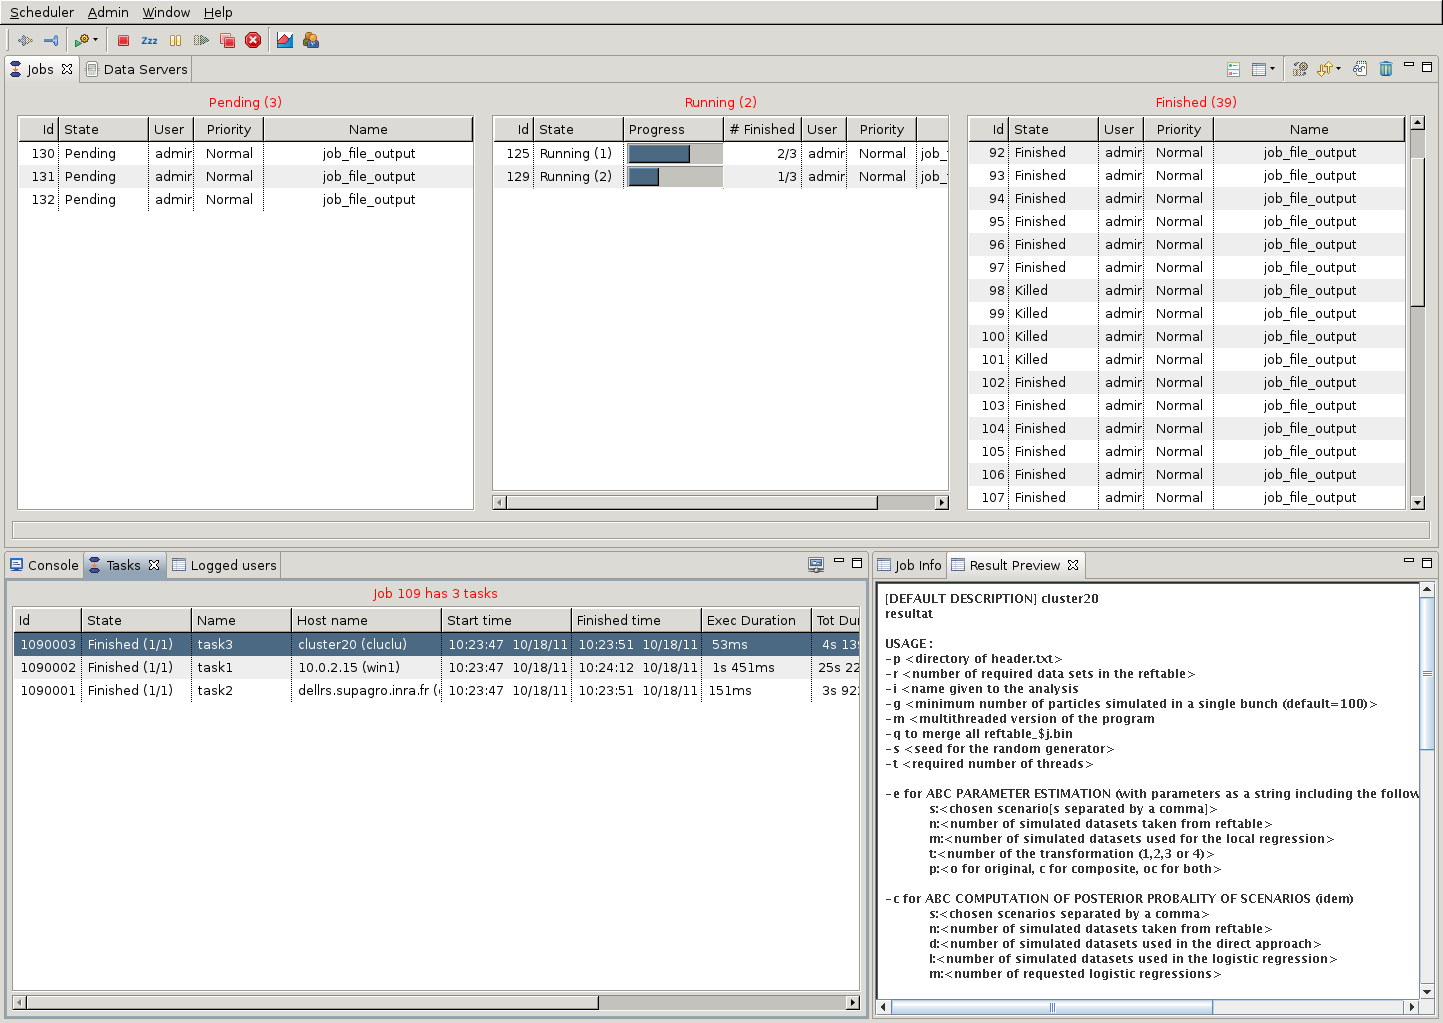
\includegraphics[scale=0.18]{sc_sched.png}
        %\caption{Principe de communication dans le réseau Proactive}
    \end{figure}
\end{frame}
\begin{frame}{Resource manager client}
    % interessant pour la partie monitoring
    \begin{figure}
        %[!bh]
        \centering
        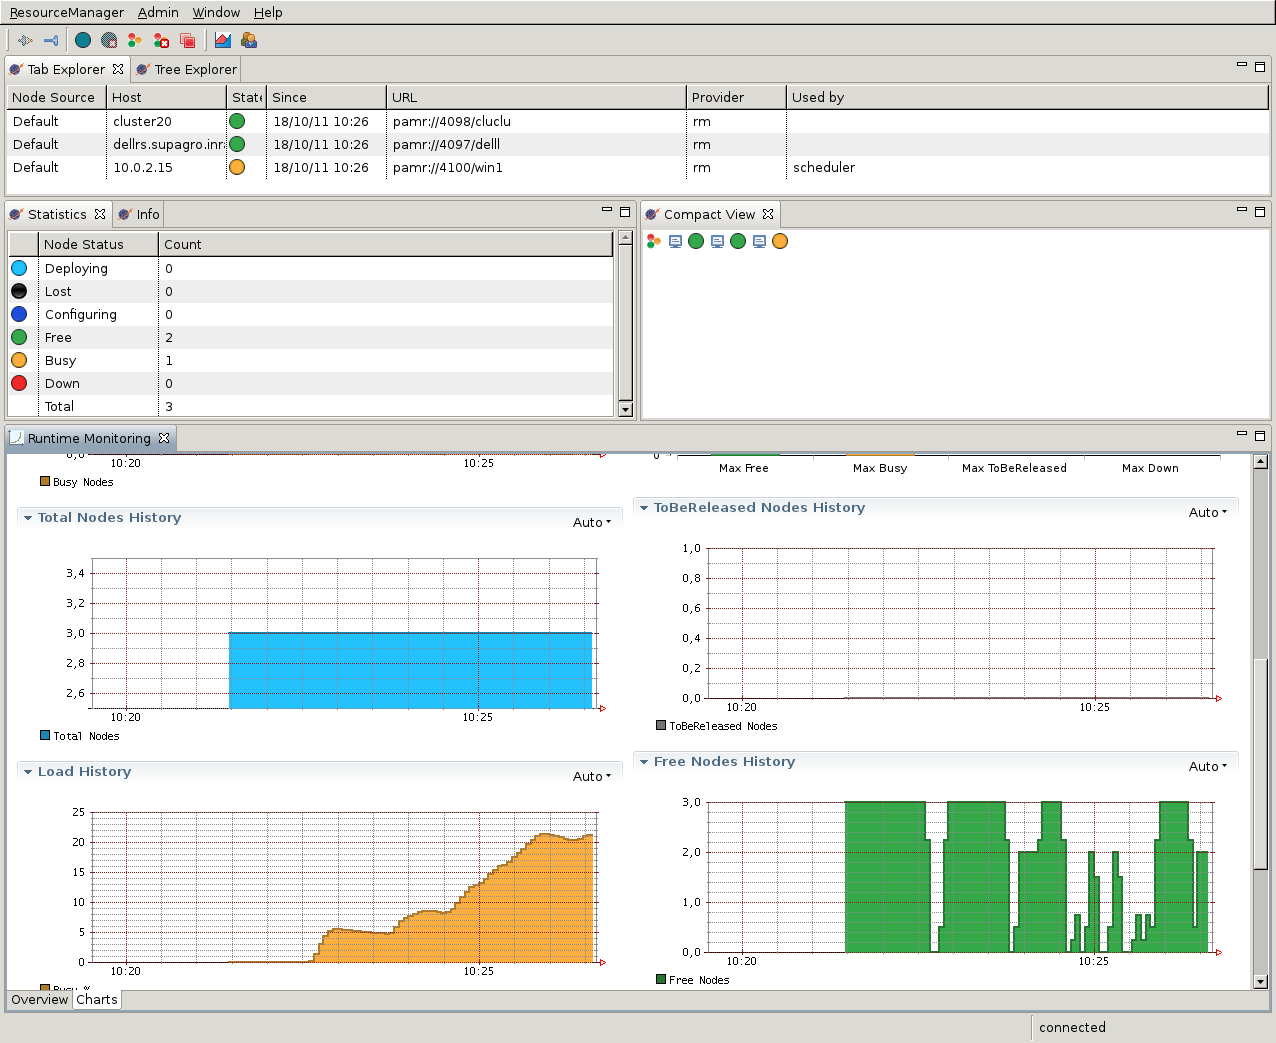
\includegraphics[scale=0.18]{sc_rmc.png}
        %\caption{Principe de communication dans le réseau Proactive}
    \end{figure}
\end{frame}


\section[Applications]{Applications possibles}
\begin{frame}
	\tableofcontents[currentsection]
\end{frame}
\begin{frame}{Intégration des ressources d'un cluster existant}
    PBS (SGE, Torque \ldots)
\end{frame}
\begin{frame}{Utiliser les postes de travail}
    Avec le programme des noeuds de calcul
    Avec les ``Agent''
\end{frame}
\begin{frame}{Utiliser les ressources d'un cloud}
    \begin{exampleblock}{Comment ?}
        Machine virtuelle dupliquée sur les noeuds du cloud qui lance 
    \end{exampleblock}
    
     On utilise la ressource dont on a besoin (pas plus pas moins) et seulement quand on en a besoin
     > pas besoin d'avoir un cluster local

     Déploiement par machines virtuelles
\end{frame}


\begin{frame}
	\begin{center}	{\huge Merci de votre attention}\end{center}
	\end{frame}
\begin{frame}
	\begin{center}	{\huge Questions}\end{center}
	\end{frame}

\end{document}
